\begin{comment}
\documentclass[10pt]{article}
\usepackage{fullpage, graphicx, url}
\setlength{\parskip}{1ex}
\setlength{\parindent}{0ex}
\title{adsr}
\begin{document}


\begin{tabular}{ccc}
The Alternative Csound Reference Manual & & \\
Previous & &Next

\end{tabular}

%\hline 
\end{comment}
\section{adsr}
adsr�--� Calculates the classical ADSR envelope using linear segments. \subsection*{Description}


  Calculates the classical ADSR envelope using linear segments. 
\subsection*{Syntax}


 ar \textbf{adsr}
 iatt, idec, islev, irel [, idel]


 kr \textbf{adsr}
 iatt, idec, islev, irel [, idel]
\subsection*{Initialization}


 \emph{iatt}
 -- duration of attack phase 


 \emph{idec}
 -- duration of decay 


 \emph{islev}
 -- level for sustain phase 


 \emph{irel}
 -- duration of release phase 


 \emph{idel}
 -- period of zero before the envelope starts 
\subsection*{Performance}


  The envelope is the range 0 to 1 and may need to be scaled further. The envelope may be described as: 


 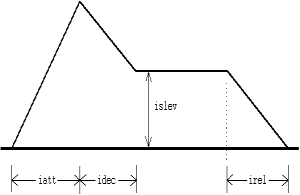
\includegraphics[scale=1]{adsr} 


 Picture of an ADSR envelope.


  The length of the sustain is calculated from the length of the note. This means \emph{adsr}
 is not suitable for use with MIDI events. The opcode \emph{madsr}
 uses the \emph{linsegr}
 mechanism, and so can be used in MIDI applications. 


 \emph{adsr}
 is new in Csound version 3.49. 
\subsection*{Examples}


  Here is an example of the adsr opcode. It uses the files \emph{adsr.orc}
 and \emph{adsr.sco}
. 


 \textbf{Example 1. Example of the adsr opcode.}

\begin{lstlisting}
/* adsr.orc */
; Initialize the global variables.
sr = 44100
kr = 4410
ksmps = 10
nchnls = 1

; Instrument #1 - a simple instrument.
instr 1
  ; Set the amplitude.
  kamp init 20000
  ; Get the frequency from the fourth p-field.
  kcps = cpspch(p4)

  a1 vco kamp, kcps, 1
  out a1
endin

; Instrument #2 - instrument with an ADSR envelope.
instr 2
  iatt = 0.05
  idec =  0.5
  islev = 0.08
  irel = 0.008

  ; Create an amplitude envelope.
  kenv adsr iatt, idec, islev, irel
  kamp = kenv * 20000

  ; Get the frequency from the fourth p-field.
  kcps = cpspch(p4)

  a1 vco kamp, kcps, 1
  out a1
endin
/* adsr.orc */
        
\end{lstlisting}
\begin{lstlisting}
/* adsr.sco */
; Table #1, a sine wave.
f 1 0 16384 10 1

; Set the tempo to 120 beats per minute.
t 0 120

; Play a melody with Instrument #1.
; p4 = frequency in pitch-class notation.
i  1  0   1  8.04
i  1  1   1  8.04
i  1  2   1  8.05
i  1  3   1  8.07
i  1  4   1  8.07
i  1  5   1  8.05
i  1  6   1  8.04
i  1  7   1  8.02
i  1  8   1  8.00
i  1  9   1  8.00
i  1  10  1  8.02
i  1  11  1  8.04
i  1  12  2  8.04
i  1  14  2  8.02

; Repeat the melody with Instrument #2.
; p4 = frequency in pitch-class notation.
i  2  16  1  8.04
i  2  17  1  8.04
i  2  18  1  8.05
i  2  19  1  8.07
i  2  20  1  8.07
i  2  21  1  8.05
i  2  22  1  8.04
i  2  23  1  8.02
i  2  24  1  8.00
i  2  25  1  8.00
i  2  26  1  8.02
i  2  27  1  8.04
i  2  28  2  8.04
i  2  30  2  8.02
e
/* adsr.sco */
        
\end{lstlisting}
\subsection*{See Also}


 \emph{madsr}
, \emph{mxadsr}
, \emph{xadsr}

\subsection*{Credits}


 Example written by Kevin Conder.
%\hline 


\begin{comment}
\begin{tabular}{lcr}
Previous &Home &Next \\
active &Up &adsyn

\end{tabular}


\end{document}
\end{comment}
